%!TEX root =  ../main.tex


\mychapters{Identities}{identities}{\chapdir/pics/PIA05380} 

Trigonometry is like the Hydra of ancient legends: you cut off one head, only to have
three more erupt out.  The interrelated nature of the circle and the reference triangle
mean there are an infinite number of ways to express the same function, via
trigonometric functions.


\newpage
\chapterminitoc


%									10 - 1
\newpage
\invisiblesection{Simple Trigonometric Equations}
\subsection{Lab}
\noindent\makebox[\textwidth]{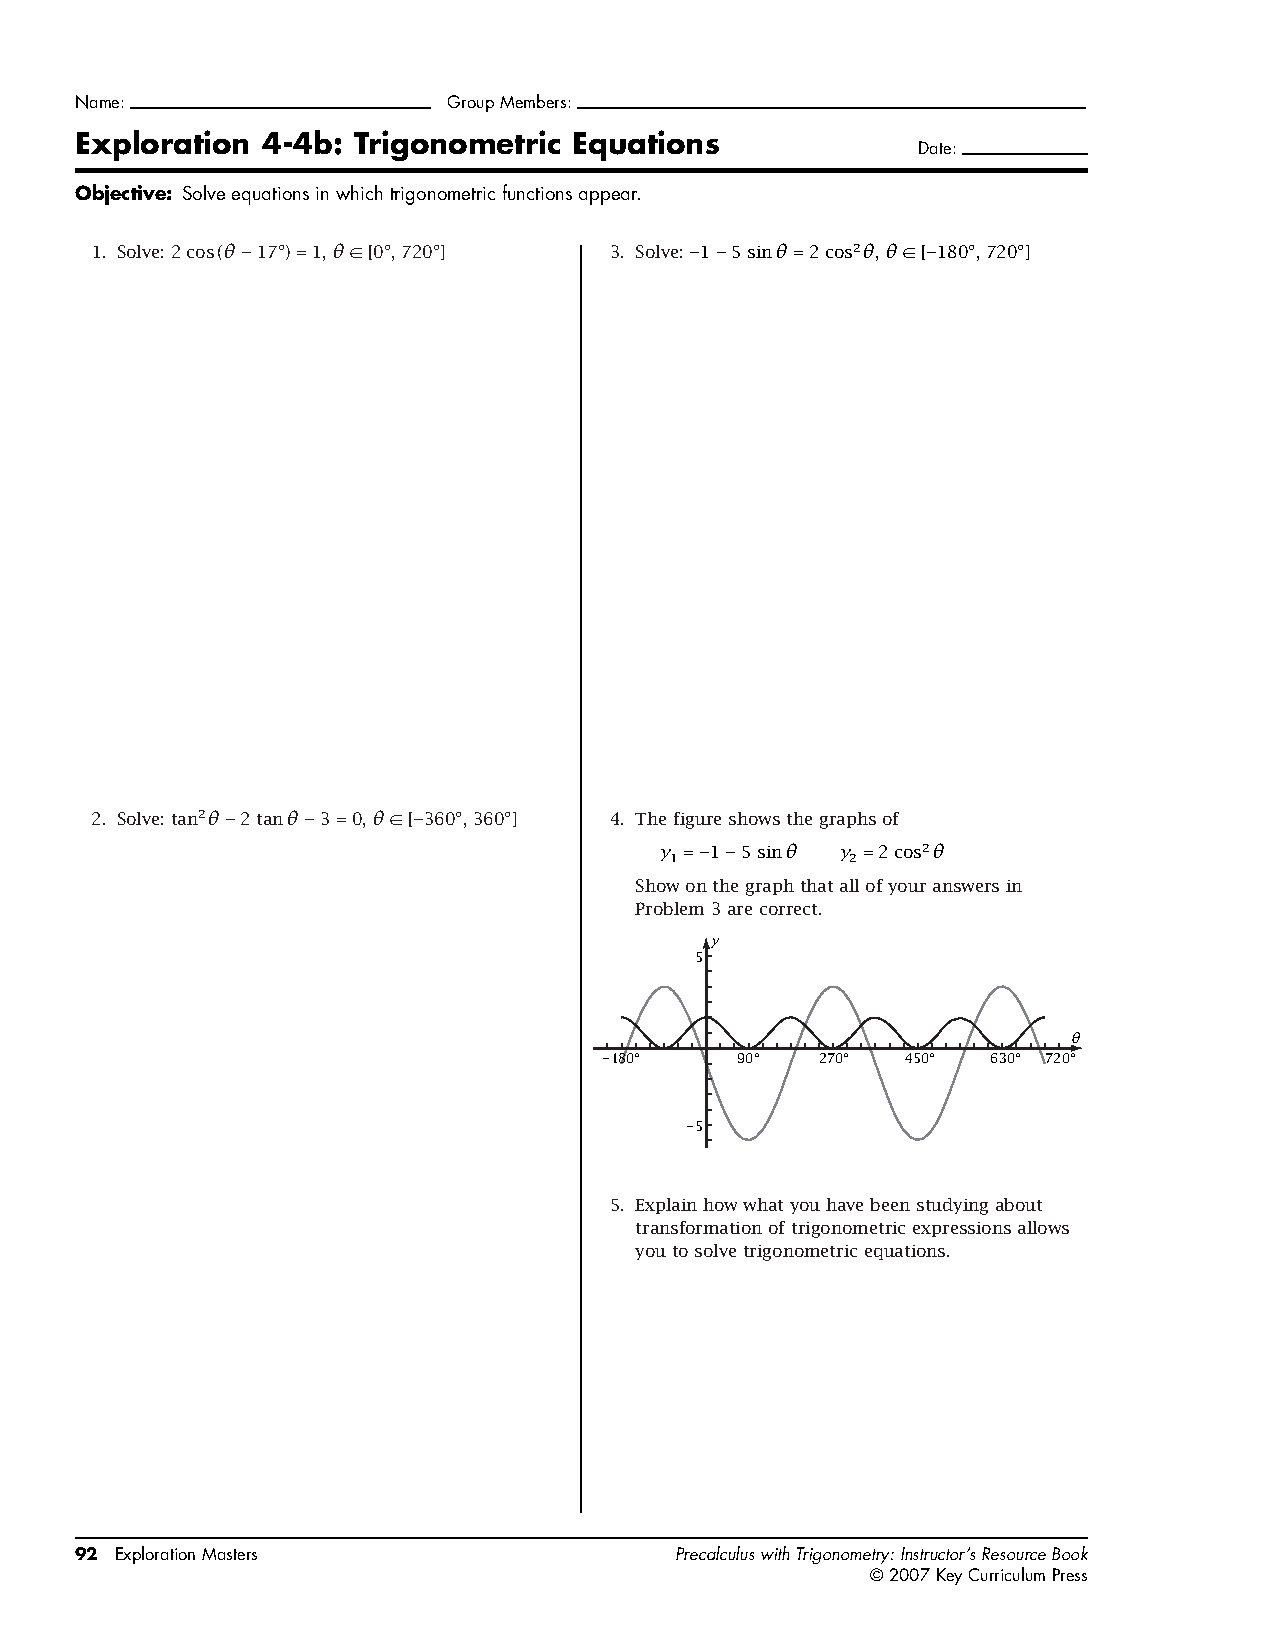
\includegraphics[width=\paperwidth]{\chapdir/1001p.pdf}}
%!TEX root =  ../main.tex

\subsection{Sine Slices}
Trigonometric equations are unlike linear equations, in that they have infinitely many
answers.  We typically answer them over a domain like $\theta \in \left[0,\tau\right]$ or
$\theta \in \left[\-\frac{\tau}{2},\frac{\tau}{2}\right]$.  Let us begin by finding a way to
express the infinite solution set.

\marginfig[-0.5in]{\chapdir/pics/Sin_unit_circle.png}{The height achieved by turning 
angle $\alpha$ will reoccur in one other place\label{fig:sinecircle}.}
Suppose we want to find all the answers to a simple equation
\begin{equation}\label{eq:sinx12}
\sin(x) = \frac{1}{2}
\end{equation}
With the Unit Circle memorized, we can easily recall that this happens at 
$\frac{\tau}{12}$.  However, we know that sine is $y$ on the Unit Circle, and so it
will come up again and again.  As Fig.~\ref{fig:sinecircle} shows, the height will
reoccur at $\frac{\tau}{2}-\theta$.  We also can add or subtract as many full-rotations
(i.e. $\tau$) as we like, and still get the same height.  This means that the full
solutions set for Eq.~\ref{eq:sinx12} is
$$
x  = \begin{cases} \frac{\tau}{12} & \pm k\tau\\
\frac{11\tau}{12} & \pm k\tau \end{cases} 
$$
where $k \in \mathbb{W}$.  Or the more general solution for $\sin\theta=x$:
\begin{equation}
\theta  = \begin{cases} \sin^{-1}(x) & \pm k\tau\\
\frac{\tau}{2} - \sin^{-1}(x) & \pm k\tau \end{cases} 
\end{equation}
Notice that only if $\sin^{-1}(x)$ is known can these be resolved without a
calculator.

\subsection{Cosine Cuts}
\marginfig[0in]{\chapdir/pics/Cos_unit_circle.png}{The horizontal displacement 
achieved by turning  angle $\alpha$ will reoccur in one other place\label{fig:cosinecircle}.}
Substitution can help prevent confusion when there are confusing extras like (e.g. $\theta-17$) inside
There can be quadratics etc, which substitution make clearer.  In general, if you find
yourself distracted or daunted by a bit of notation, remove it from sight for a moment and
solve the easier part, before bringing back the difficulty.

Consider the broad question, asked without domain restrictions
\begin{equation}
\cos(x) = -\frac{1}{2}
\end{equation}
This should be read in our minds in a clear verbal language as, ``What angles $x$ can be
turned from standard position the produce horizontal displacements of 0.5 to the left?''
Hopefully, this restatement allows us to visualize that both a third and fourth
quadrant angle exist that have the same $x$ value.  Because these angle can be reached by
turning the same amount clockwise or counter-clockwise, we can write our answer
succinctly as 
$$
x= \pm\frac{\tau}{3} \pm k\tau
$$
Universally, the solution to $\cos\theta = x$ is
\begin{equation}
\theta = \pm\cos^{-1}(x) \pm k\tau
\end{equation}

Now, if we are solving an equation with a strange term, we are still able to see the
answers clearly through substitution.  For example, 
$$
2 \cos (\theta - 17^\circ) = 1
$$
invites us to divide by two, but what then?  It is clarifying to substitute in the expression
\begin{equation}
u = \theta - 17
\end{equation}
A perfectly valid move, provided with undo it before the end.  If $\cos u = \frac{1}{2}$, our
answers in degrees are $u = \pm60^\circ \pm k\tau$, but we have answered in the wrong
variable.  ``Unsubstituting'', we get
\begin{equation}
\theta - 17^\circ = \begin{cases} 60^\circ & \pm k\tau \\ -60^\circ & \pm k\tau \end{cases}
\end{equation}
Perhaps you have not experienced manipulated equations with cases in them.  It is no
surprise that we simple add 17 to both sides, only on the right there are two places to do so.
Final answers:
$$
\theta = \begin{cases} 77^\circ & \pm k\tau \\ -43^\circ & \pm k\tau \end{cases}
$$

\subsection{Tangent Tilts}
Lastly, tangent can be the easiest to deal with, because it's period is less than one
full rotation.  Thinking back to the unit circle, slopes are the same in the first and third
quadrant, and again in the second and fourth.  This is because any line passing through
the origin is identical if rotated $\frac{\tau}{2}$.  

\begin{example}
	\exProblem
Factor and solve $\tan^2\theta - 2\tan\theta - 3 = 0$ for all it solutions.

	\exSolution
If it is not obvious that this is a quadratic in tangent, we can substitute $u = \tan\theta$ to
get $u^2 - 2u - 3 = 0$, and un-substitute later.  This factors easily into $(u-3)(u+1)=0$, which
means $u = \{3, -1\}$.  Asking when tangent equals -1 is the same as asking, ``For what
angles is the slope -1?''  These are all the angles beginning with a $\frac{\tau}{8}$ reference
angle in the second quadrant, and every half-rotation after that, i.e. $\frac{3\tau}{8}+\frac{\tau}{2}k$.
The angle of a slope of 3 is not a rational number, but the TI-8* says it is approximately
1.25, so we can write $1.25 + \frac{\tau}{2}k$.
\end{example}


The period can be off, so consider making a general solution and using it to generate answers

\newpage
\subsection{Exercises}
to be done in Kuta


%									10 - 2
\newpage
\section{Co-function, Pythagorean, Even/Odd}
\subsection{Problems}
To be done in Word.
Count sides as sin, cos, 1.  Pythagorus
Draw right triangle.  Use theta and 90-theta.  Side of x, y, r.  find sine and cosine of each
\newpage
%!TEX root =  ../main.tex

\subsection{Reference Triangle Within}
\subsection{Reference Triangles Without}
\subsection{Full Geometry}
\subsection{Algebra Ratios}
\subsection{Time Savers}
\subsection{Conjugates}

\newpage
\subsection{Exercises}
Use the Pythagorean identities to produce/solve ellipses and hyperbolas - to be do


%									10 - 3
\newpage
\invisiblesection{Sum and Difference Identities}
\subsection{Problems}
Make rectangles in Word --- to be done
\subsection{Cosine Sum and Difference}
\subsection{Sine Sum and Difference}
\subsection{Tangent Sum and Difference}
\newpage
\subsection{Exercises}
to be done in Kuta


%									10 - 4
%\newpage
\invisiblesection{Double Angles}
\subsection{Problems}
\noindent\makebox[\textwidth]{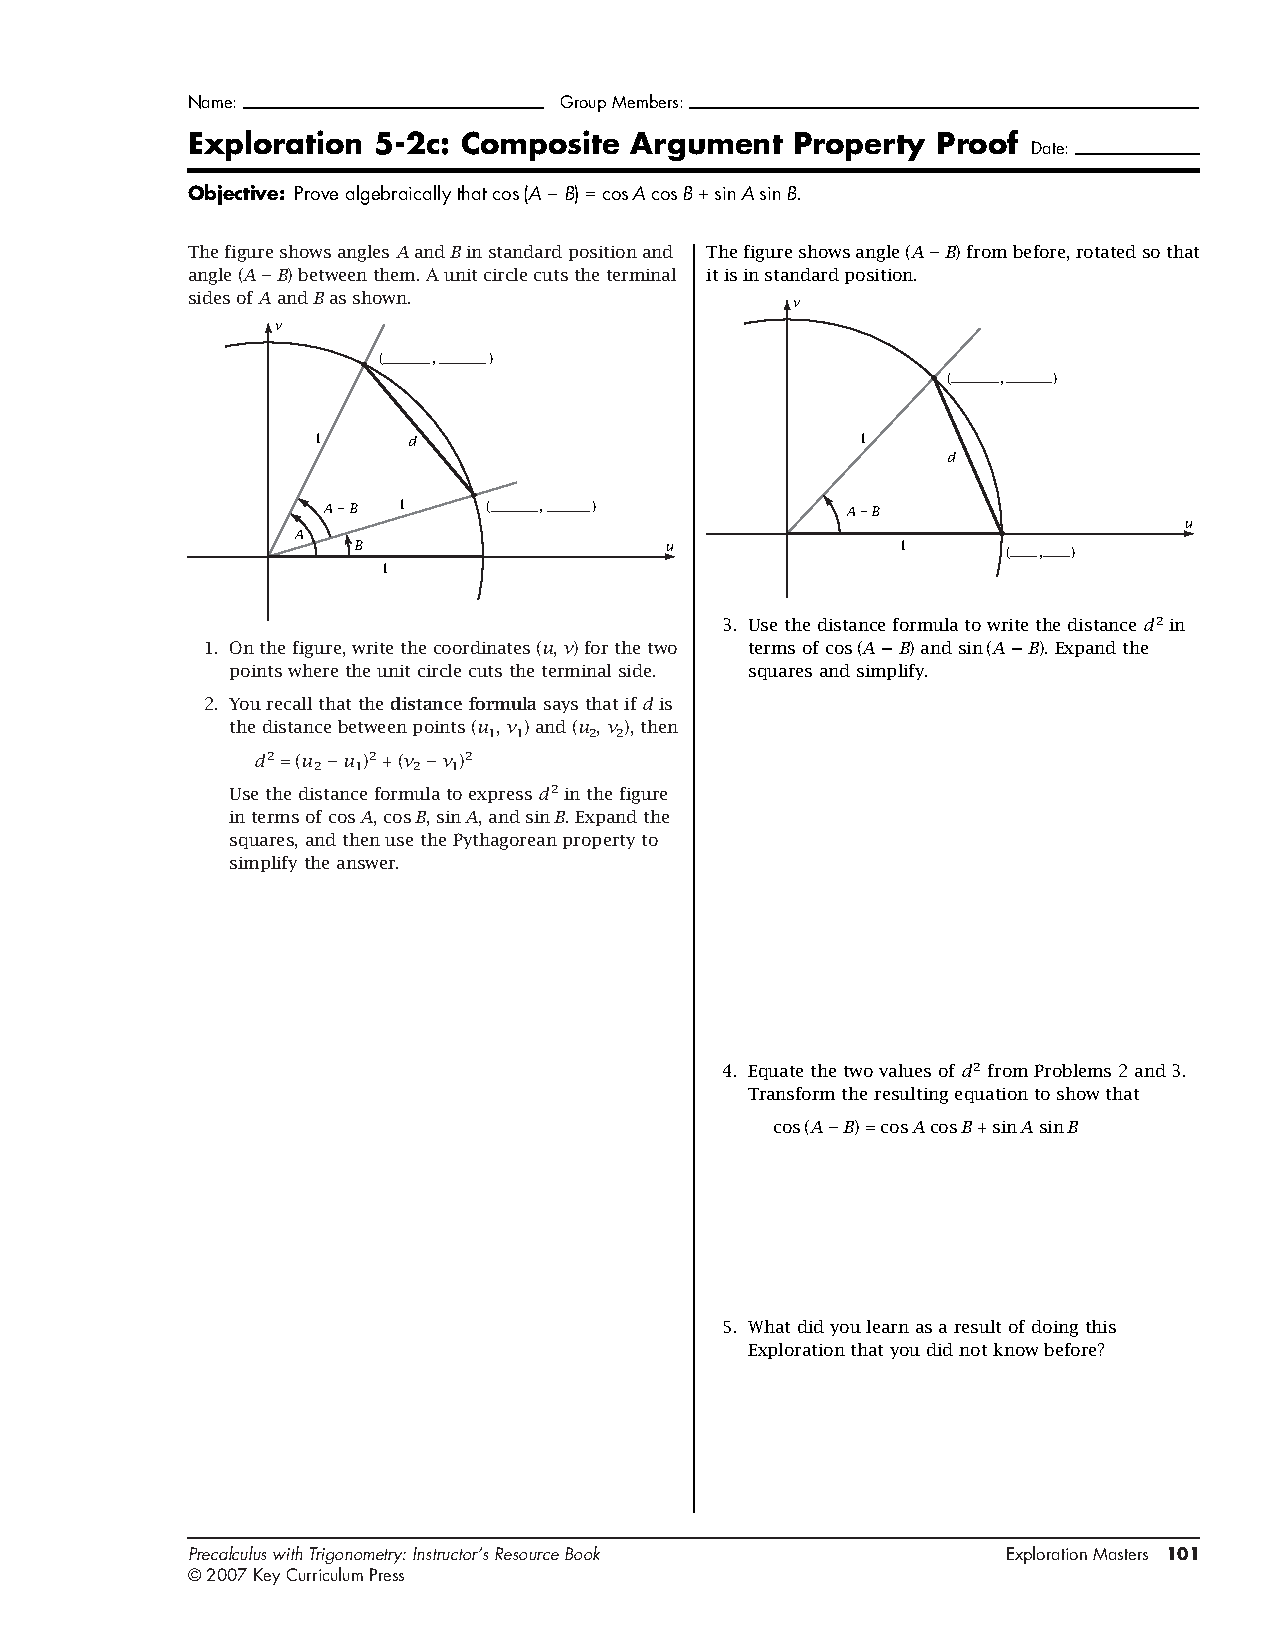
\includegraphics[width=\paperwidth]{\chapdir/1004p.pdf}}
\subsection{Double Sine}
\subsection{Double Tangent}
\subsection{Double Cosine}
\subsection{Half and Power}
\newpage
\subsection{Exercises}
to be done in Kuta


%									10 - 5
\newpage
\section{Proofs}
\subsection{Problems}
to be done in word
\newpage
\subsection{Summary of Trigonometric Derivatives}
\subsection{Summary of Trigonometric Integrals}
\subsection{Summary of Trigonometric Identities}
\subsection{Techniques for Proofs}
\newpage
\subsection{Exercises}
Prove that the area of a circle is pi r squared
\index{area!of a circle as an integral}
Prove that the area of an ellipse with radii a, b is abpi
\index{area!of an ellipse as an integral}
to be done in word


\newpage
\section{Review}
\subsection{Chapter Review}
\subsection{Chapter Test}